% =====================================================================
% Snippet: layer-stack.tex
% =====================================================================
% USAGE: "N=6 layers" repetition stack — grey semi-transparent boxes
% behind the main box to suggest "this layer repeats N times".
% Used in examples 06 Transformer (Encoder Layer ×6 / Decoder ×6).
%
% Copy %% COPY-START / END, replace:
%   - main_box: the front main box (its content + style)
%   - stack_count: N (number of layers, default 4-6 visible)
%   - offset_x, offset_y: shift per layer (default 0.15)
%   - origin_x, origin_y: anchor of front box
%   - layer_label: "N=6 layers" or "×12" text
% =====================================================================

\documentclass[tikz,border=10pt]{standalone}
\usepackage{xcolor,tikz}
\usetikzlibrary{positioning,calc}

\definecolor{acaBlueLine}{HTML}{3060A8}
\definecolor{acaBlueFill}{HTML}{DCE6F4}
\definecolor{acaGreyLine}{HTML}{606060}

\begin{document}
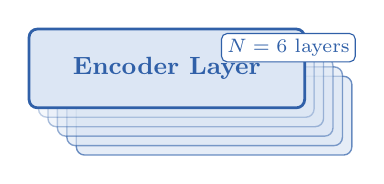
\begin{tikzpicture}

%% COPY-START =========================================================

\def\xO{0}
\def\yO{0}
\def\boxW{3.5}
\def\boxH{1.0}
\def\stackN{5}              % visible layers in stack (besides front)
\def\offsetX{0.12}
\def\offsetY{-0.12}
\def\layerLabel{$N = 6$ layers}

% --- BACK LAYERS (drawn first, light + transparent) ---
% Each successive layer slightly more transparent
\foreach \i in {\stackN,...,1} {
  \pgfmathsetmacro\op{20 + 10*\i}    % 30-70% opacity
  \pgfmathsetmacro\sx{\xO + \i * \offsetX}
  \pgfmathsetmacro\sy{\yO + \i * \offsetY}
  \fill[acaBlueFill, opacity=\op/100, rounded corners=3pt]
    (\sx, \sy) rectangle (\sx + \boxW, \sy + \boxH);
  \draw[acaBlueLine, opacity=\op/100, line width=0.5pt, rounded corners=3pt]
    (\sx, \sy) rectangle (\sx + \boxW, \sy + \boxH);
}

% --- FRONT MAIN LAYER (solid) ---
\fill[acaBlueFill, rounded corners=3pt]
  (\xO, \yO) rectangle (\xO + \boxW, \yO + \boxH);
\draw[acaBlueLine, line width=1.0pt, rounded corners=3pt]
  (\xO, \yO) rectangle (\xO + \boxW, \yO + \boxH);
\node[anchor=center, font=\small\bfseries, color=acaBlueLine]
  at (\xO + \boxW/2, \yO + \boxH/2)
  {Encoder Layer};

% --- "×N layers" badge (top-right corner) ---
\node[anchor=north east, font=\scriptsize, color=acaBlueLine,
      fill=white, draw=acaBlueLine, line width=0.4pt,
      rounded corners=2pt, inner sep=2pt]
  at ($(\xO + \boxW, \yO + \boxH) + (\stackN*\offsetX + 0.05, -0.05)$)
  {\layerLabel};

%% COPY-END ===========================================================

\end{tikzpicture}
\end{document}
